\documentclass[twocolumn]{article}

\usepackage[english]{babel}

\usepackage{graphicx}
\graphicspath{{figs/}}

\usepackage{amsmath}

\usepackage{tikz}
\usetikzlibrary{shapes}

\usepackage{hyperref}
\usepackage{subcaption}

\usepackage[draft, footnote, margin=false]{fixme}

\newcommand{\ie}{{\textit{i.e.\ }}}
\newcommand{\cf}{{\textit{cf\ }}}
\newcommand{\eg}{{\textit{e.g.\ }}}
\newcommand{\al}{{\textit{et al.\ }}}

\newcommand{\M}[3]{{\mathcal{M}(#1, #2, #3)}}
\newcommand{\model}[3]{{$\mathcal{M}(#1, #2, #3)$}}
% generic mutual model (gmodel) 
\newcommand{\gmodel}[2]{{$\mathcal{M}(#1, #2)$}}
\newcommand{\refmodel}[2]{{$\mathcal{M}(#1, #2)$}}
\newcommand{\Model}[3]{{$\mathcal{M}^{\circ}(#1, #2, #3)$}}
\newcommand{\gModel}[2]{{$\mathcal{M}^{\circ}(#1, #2)$}}
\newcommand{\Mdeg}[3]{{\mathcal{M}^{\circ}(#1, #2, #3)}}
\newcommand{\gMdeg}[2]{{\mathcal{M}^{\circ}(#1, #2)}}

\newcommand{\groundingcriterion}{{$\mathcal{M}^{\circ}_{min}$}}
\newcommand{\inigrounding}{{$\mathcal{M}^{\circ}_{t_0}$}}

\newcommand{\concept}[1]{{\small \texttt{#1}}}
\newcommand{\stmt}[1]{{\footnotesize \tt $\langle$ #1\relax$\rangle$}}


\title{Is Partner Modeling Mutual?}

\begin{document}
\maketitle

\begin{abstract}
    TDB
\end{abstract}

\section{Introduction}


From its very beginning, CSCL research has been following Roschelle \& Teasley's
(1986) suggestion that collaborative learning has something to do with the
process of constructing and maintaining a shared understanding of the task at
hand. Building a shared/mutual understanding refers to the upper class of
collaborative learning situations, those in which students should build upon
each other's understanding to refine their own understanding. What is expected
to produce learning is not the mere fact that two students build the same
understanding but the cognitive effort they have to engage to build this shared
understanding (Schwartz, 1995). This effort can be observed by the frequency of
rich interactions, \ie interactions whose occurrence has been related to
learning: (self-) explanations in cognitive science (Chi ; Webb), conflict
resolution in socio-cognitive theories (Doise), mutual regulation (Blaye,) in a
Vygostkian perspective, etc. The construction of a shared understanding has been
investigated for several years in psycholinguistics, under the  notion of
“grounding” (Clark \&Wilkes-Gibbs, 1986). However, the relevance of grounding
mechanisms for explaining learning outcomes has been questioned. The monitoring
and repair of mis-understanding explains for instance referential failures in
short dialogue episodes but does hardly predict conceptual change over longer
sessions (Dillenbourg \& Traum, 2006). The cumulative effect of grounding
episodes can probably be better understood from a socio-cultural perspective:
"collaborative learning is associated with the increased cognitive-interactional
effort involved in the transition from learning to understand each other to
learning to understand the meanings of the semiotic tools that constitute the
mediators of interpersonal interaction" (Baker, Hansen, Joiner \& Traum, 1999).
Several scholars suggest that CSCL research should go deeper in the
understanding of how partners engage into shared meaning making (Stahl, 2006) or
'intersubjective' meaning making (Suthers (2006).  

Paradoxically, while Clark's theory is somewhat too linguistic from a conceptual
change viewpoint, it is criticized at the same time as being too cognitivist by
some psycholinguists, \ie as overestimating the amount shared knowledge and
mutual representations actually necessary to conduct a dialogue. The fundamental
issue, as old as philosophy, is the degree of coupling between the different
levels of dialogue, mostly between the lexical / syntactical level and the
deeper semantic levels. Pickering \& Garrod (2004) argue that the mutual
understanding starts mostly with a 'local alignment' at the level of the
linguistic representations, due to priming mechanisms, and that this superficial
alignment may – in some cases- lead to a 'global alignment' of the semantic
level.  For these authors, the convergence in dialogue, and even the repair of
some misunderstandings, is explained by this mimetic behavior more than by a
monitoring of each other's knowledge: "…interlocutors do not need to monitor and
develop full common ground as a regular, constant part of routine conversation,
as it would be unnecessary and far too costly. Establishment of full common
ground is, we argue, a specialized and non-automatic process that is used
primarily in times of difficulty (when radical misalignment becomes apparent)."
(p. 179). This view is actually not incompatible with Clark's grounding
criterion (REF): the degree of shared understanding that peers need to reach
depends upon the task they perform. For instance, a dialogue between two
surgeons might rely on superficial alignment if they talk about their friends
but has to guarantee accurate common grounds when talking about which
intervention will be conducted in which way on which patient.  Some CSCL
scholars stressed the 'illusion of shared understanding' (JACCO?), \ie the
potential decoupling between linguistic alignment and actual shared meanings.

This interesting cognitive science debate mostly occurred outside the field of
learning. In education, the question is to relate these mechanisms to learning
outcomes. Is linguistic alignment sufficient to trigger conceptual change? Does
negotiation of meaning only occurs when partners monitor and diagnose each
other's knowledge. If the ratio between shallow alignment and deep grounding
depends upon the task, and if deep grounding is a condition for learning, then
the pedagogical challenge is to design tasks that require deep grounding. Most
empirical studies on grounding and alignment are conducted with tasks, which
despite being qualified as 'ecologically valid' by their authors, are mere
referencing tasks such as asking the way to the train station or helping the
peer to choose a picture among many. In this contribution, we explore several
richer tasks such as arguing on a sensitive issue or building a concept map.  

Deep grounding or shared meaning making requires some cognitive load. For Clark
\& Wilkes-Gibbs (1986), what is important is not the individual effort made by
the receiver of a communicative act, but the overall least collaborative effort.
The cost of producing a perfect utterance may be higher than the cost of
repairing the problems that may arise through misunderstandings. For instance,
subjects are less careful about adapting their utterances to their partner when
they know they can provide feedback on his/her understanding (Schober, 1993). We
introduced the notion of ‘optimal collaborative effort' (Dillenbourg et al,
1996) to stress that misunderstanding should not be viewed as something to be
avoided (if this was possible), but as an opportunity to engage into
verbalization, explanation, negotiation, and so forth. This issue is related to
the global argument regarding cognitive load in learning activities, especially
in discovery learning environments: there is no learning without some cognitive
load, but overload may hinder learning (Paas, Renkl \& Sweller, 2003). In the
context of collaborative learning, we understand the cognitive load induced by
mutual modeling as part of Schwartz's (1995) notion of effort towards a shared
understanding. For instance, CSCL researchers expanded the use of 'collaboration
scripts' (Aronson,?). A script is a pedagogical method that collaborative
learning activities in order to foster the emergence of productive interactions
such as argumentation, explanation or conflict. Conflict-resolution scripts such
as the ArgueGraph (Dillenbourg \& Hong, 2008) forms pair of students with
opposite opinions, which increases the difficulty of consensus building,
requiring more justifications, more negotiation, more load. Similarly, JIGSAW
scripts provide peers with different but complementary knowledge for augmenting
(reasonably) the effort group members have to engage to reach a shared solution. 

%\paragraph{Theory of Mind}
%
%Theory of Mind (originally defined in~\cite{premack1978does}) is the cognitive
%ability that a subject possesses to represent the mental state of another
%agent, possibly including knowledge that contradicts the subject's own model: for
%example, a book can be at the same time \emph{visible} for myself, and \emph{not
%visible} for you.
%
%Children develop this skill, which is essential to understand others'
%perspectives during interactions, around the age of three. It supposes the
%ability to build, store and retrieve separate models of the knowledge of the
%interactors.
%
%One classical application of this cognitive skill is the so-called
%\emph{False-Belief} experiment (also known as the \emph{Sally and Ann}
%experiment)~\cite{Leslie2000}: a child is asked to watch a scene where two
%people, A and B, manipulate objects. Then A leaves and B hides away one
%object. When A comes back, we ask the child ``where do you think A will
%look for the object?''. Before acquiring a theory of mind, children are not
%able to separate their own (true) model of the world (where they know that
%the object was hidden) from the model of A, which contains \emph{false
%beliefs} on the world (A still thinks the object is at its original
%position since he did not see B hiding it).

\section{Mutual Modeling}


In order to build a shared understanding, do partners have to build a
representation of each other's knowledge? We refer to \emph{mutual modeling} as
the process of inferring one's partner mental states. Any claim that students
carry out a detailed monitoring of their peers would be as incorrect as any
claim that they do not maintain any representation at all. If mutual modeling
had to be permanently detailed and accurate, subjects would obviously face a
huge cognitive load. Conversely, peers could not collaborate without some
minimal amount of mutual modeling. For instance, A cannot disagree with B
without knowing that B has a different opinion. The mutual model can be implicit
(A is not aware of what he knows about B), by-default (I believe that B beliefs
what I believe unless contrary evidence), opportunistic (A does not model B
unless the conversation requires it), global (A infers B's beliefs based on
categories such as age, culture or profession) and, of course, it can be
incorrect… but it can not remain empty. Dialogues include many instances of
utterances such as "I thought he would do that" (first level of mutual
modelling) or even "He thought I would do that but I intended something else."
(second level of mutual modelling).

The content of mutual models ranges from 'dispositional' versus 'situational'
aspects. The 'dispositional' aspects refer to A's representation of B's long
term knowledge, skills or traits. It is thus closely related to the notion of
transactive memory~\cite{wegner1987transactive, moreland1999transactive}.
'Situational' aspects refer to A's representation of B's knowledge, behavior or
intentions specifically activated in the situation in which A and B are
collaborating, some of them being valid for 2 seconds, other ones for 2 hours.
Here are examples of fragments that constitute A's model of B regarding to
aspects X, noted $Model(A,B,X)$:

\begin{itemize}

    \item $Model(A,B, knowledge)$: What does A know about B's knowledge with
        respect to the task at hand or, inversely, about B's knowledge gaps?
        When can A consider B's statements as reliable? 

    \item $Model(A,B, skills)$: What does A know about B's skills with respect to
        the task at hand? May A expect B to perform well in a specific subtask?
        The effectiveness of division of labor depends on the quality of this
        mutual model. 

    \item $Model(A,B, goals)$: What does A know about B's intentions with respect
        to the project, including B' motivation and commitment? Can A trust B
        when B promises to deliver? 

    \item $Model(A,B, task)$: What does A know about B's representation of the
        situation and the task: does A knows whether B has the same
        understanding of the problem at stake? 

    \item $Model(A,B, plans)$: What does A know about B's strategy. Does A
        understand why B did what he did? Is A able to anticipate what B will do
        next? 

    \item $Model(A,B, "urgent")$: What does A about know B's understanding of A's
        last utterance: does ‘urgent' means now, ASAP and ‘not too lat' ?

    \item We could continue the list of what is X is \model{A}{B}{X}: beliefs,
        emotions, history, status, …

\end{itemize}

We have different levels of mutual modelling. If A states "B thinks I am god in maths", we
are the second level of mutual modelling:  $Model(A, B, Model(B,A, knowledge="good in
math"))$. There is an infinite regress of nested models: If A says "B knows that
I don't expect him to solve this statistics problem" corresponds to $Model(A, B,
Model (B, A (Model (A,B, statistic-skills)))$.

A partner model is probably not a "box", \ie not a monolithical representation
but rather a mosaic of information fragments about the partner, with various
grain sizes and various life cycles. This mosaic is elaborated through various
mechanisms, first for building an initial model of the partner and then for
updating this model.  As two students meet for the first time, mutual models are
initialized by the assumptions they make upon each other from cues such as
his/her membership to large categories (age, culture, profession, ...) include
stereotypes (sportsmen, junkie, business women, Swiss,...) as well as physical
appearance. Scholars studied how initial modeling impacts communication. In
their experiments on initial mutual modelling, Slugoski, Lalljee, Lamb \&
Ginsburg~\cite{slugoski1993attribution} pretended to their subjects that their
(fake) partner had or had not received the same information. They observed that
the subjects adapted their dialogue by focusing the explanation on the items
that (s)he was supposed to ignore. Brennan (1991) \fixme{ref} showed that the subjects used
different initial strategies in forming queries depending on who they were told
their partner was.  

Initial common grounds are also initiated by co-presence: they include events to
which A and B attended together~\cite{clark2002definite} in the physical space
or in our cultural space (\eg ‘09-11'). Co-presence means that we can refer to
a shared objects and event,-s it does of course not imply that we give them the
same meaning. Namely, a shared screen does not mean a shared
understanding~\cite{dillenbourg2006sharing}.

After initialization, mutual models are updated along the collaborative work
through verbal and non-verbal interactions. A default inference rule is that "my
partner agrees with me unless he disagrees", which reject the critiques that
mutual modeling generates an unbearable cognitive load. This default rule is
superseded by the several mechanisms for monitoring and repairing one's partner
understanding: acknowledgement, continuous attention, relevance of next turns,
facial expressions including gaze signals, etc.

Mutual modeling does not occur in a vacuum but it is highly contextualized. REF
reviews the features of the collaborative situation, namely the media
(cotemporality… ), may facilitate or hamper mutual modeling. Hutchins (SILENCE)
reported a study in which a short silence between two pilots was perfectly
interpreted because it occurred in a highly constrained communication context.
Some environments are more productive than others in helping peers to detect
their misunderstandings. Roschelle~\cite{roschelle1995construction} reformulate
the design of CSCL interfaces as providing ways for peer to detect and repairs
their misunderstanding. In CSCW, researchers have explored various so-called
"awareness tools", \ie functionalities that inform A is about B's actions that A
could not directly perceived because B was working on a different subset of the
virtual space. Different awareness tools will be addressed in this contribution
since they allowed us to manipulate experimentally the mutual modelling activity. 


%\subsection{State of the Art}
%
%\paragraph{Building a model of a human during the interaction} Perspective
%Taking is a human ability which allows one to put him/herself in another
%person's point of view. Studied in psychology
%literature~\cite{Flavell1992,Tversky1999}, this ability is crucial when
%interacting with people by allowing one to reason on others' understanding of
%the world in terms of visual perception, spatial descriptions, affordances and
%beliefs, etc.  In the last years these notions have been gradually employed in
%HRI.~\cite{Breazeal2006} presents a learning algorithm that takes into account
%information about a teacher's visual perspective in order to learn a task.
%~\cite{Johnson2005} apply visual perspective taking for action recognition
%between two robots.~\cite{Trafton2005} use both visual and spatial perspective
%taking to find out the referent indicated by a human partner.
%
%The cognitive model that the robot builds for the agent it interacts with is
%still simple and mostly focused on geometric features (who sees what? What are
%our relative positions? etc.). Extending this knowledge with more subtle
%perceptions (emotional state for instance) remains to be done.
%
%\paragraph{Joint action}
%Several theories dealing with collaboration~\cite{Cohen1991,Grosz1996,Clark1996}
%emphasize that collaborative tasks have specific requirements compared to
%individual ones, \eg, since the robot and the person share a common goal, they
%have to agree on the manner to realize it, they must show their commitment to
%the goal during execution, etc. Several robotic systems have already been built
%based on these theories~\cite{Rich1997,Sidner2005,Breazeal2003} and they all
%have shown benefits of this approach. They have also shown how difficult it is
%to manage turn-taking between communication partners and to interleave task
%realization and communication in a generic way. Finally, today only few
%systems~\cite{Fong2006,Breazeal2003,Sisbot2008} take humans into account at all
%levels.
%
\section{A model for mutual modelling evaluation}

To report experiments on mutual modeling, we suggest
the notation \model{A}{B}{X} to denote ``A knows that B knows X". This is a
simple but useful reduction to reason on mutual modelling. This
notation does not mean A has an explicit, monolithic representation of B: it
must be understood as an abstraction referring to complex socio-cognitive
processes. Besides, we refer to the \emph{degree of accuracy} of the model as
\Model{A}{B}{X}.

We parametrize and assess the mutual modelling effort through 3 variables:

\begin{enumerate}

    \item Tasks vary a lot with respect to how much they require.  The grounding
        criterion -- denoted \groundingcriterion -- refers to how
        important it is to mutually share a piece of information X to succeed
        the task T. It can be computed as the probability to succeed T despite
        the fact X is not grounded. $\mathcal{M}^{\circ}_{min}(A,B,X)$ can be
        estimated from the correlation between \Model{A}{B}{X} and task
        performance. 

    \item Before any specific grounding act, there is usually a non-null probability
        that X is mutually understood by A and B: because X is part of A's and
        B's cultures, because it is manifest to co-present subjects or simply
        because there is not much space for misunderstanding or disagreement
        about X. We could not simply collaborate without a high level of initial
        grounds. We note the theoretical accuracy of initial grounds:
        $\mathcal{M}^{\circ}_{t_0}(A,B,X)$.

    \item The cost of grounding X refers to the physical and cognitive effort
        necessary to perform a grounding act $\alpha$: a verbal repair (\eg
        rephrasing), a deictic gesture, a physical move to adopt one partner's
        viewpoint, etc. This cost varies according to media features ( Clark \&
        Brennan (REF)). 

\end{enumerate}

Based on these 3 parameters, the probability of making an action $\alpha_{t_1}$ about
content X at time $t_1$ during task T in order to increase \Model{A}{B}{X}
at time $t_2$ is the ratio between how much it is needed  ((2)-(1)) and how much it
costs (3)~\cite{traum1996miscommunication}:

\begin{multline} \label{eq:probrepair}
p(\alpha_{t_1}(X,T) / M^{\circ}_{t_2}(A,B,X) \nearrow) \approx \\
\frac{(M^{\circ}_{min}(A,B,X,T) - M^{\circ}_{t_1}(A,B,X))}{cost (\alpha)}
\end{multline}

This is qualitative summary more that a real equation since several parameters
are hard to quantify (\eg the cost an communication acts depends upon the user
as well) but it clarifies the parameters of the experiments we propose hereafter.

\begin{itemize}
    \item \Model{A}{B}{X}: Our experiments address different contents that can be
        represented in mutual models:

    \begin{enumerate}
        \item \model{A}{B}{emotion}: how accurately A perceives B's emotional state
            (study 3); 

        \item \model{A}{B}{actions} is about how well A guesses what action B has
            done (study 2) or will do next  (study 1)

        \item \model{A}{B}{knowledge}: how accurately A estimates B's knowledge
            with respect to the material they learn together (study 4 and 5)

    \end{enumerate}



    \item \Model{A,B}{X}{T} Our studies concern various collaborative tasks:
        argumentation (study 3), games (study 1 and 2) and concept mapping
        (study 4 and 5). By varying the tasks, we do actually vary the grounding
        criterion but they all require a "reasonably high" grounding criterion.
        All tasks are about building a solution or a representation together; we
        did not address everyday conversations. 

    \item $\mathcal{M}^{\circ}_{t1}(A,B,X)$ Along the same reasoning, the initial degree
        of common grounds should be rather low (and hence the difference between
        initial and required degrees rather high) in order to make mutual
        modelling effort more observable. Studies 1, 4 and 5 have been conducted
        with teams of students who did not know each other. They came
        nonetheless from the same university: they hence had some general common
        grounds.  For studies 2 and 3, students knew each other before for
        reasons explained later on. In study 5, we manipulated the initial mutual modelling by
        using a JIGSAW script.

    \item $cost(\alpha)$ In all studies but study 4, the cost of  grounding is
        an independent variable. Study 3 uses media richness as independent
        variable, with the hypothesis that modeling emotions is "cheaper" with a
        richer medium, \ie  when peers can see each other.  Studies 1,2 and 4
        use awareness tools which, in principle, reduce the cost of mutual modelling, but do
        not eliminate all costs: if the tool provide A with information about
        what B does/knows, this additional information may actually increase
        cognitive load. Awareness tools constitute as a kind of mutual modelling prosthesis,
        and, like any prosthesis, they many augment mutual modelling (by facilitating it or
        even scaffolding it) or inhibit it (by making it useless).

\end{itemize}


Each of the studies that we present in the next section have been design in such a way that, while tractable on a
robot, mutual modelling plays a key role for the task performance: the tasks
require a ``reasonably high'' grounding criterion \groundingcriterion,
and all tasks are about building a solution or a representation together.

Along the same reasoning, the initial degree of common grounds \inigrounding
should be rather low (and hence the difference between initial and required
degrees rather high) in order to make mutual modelling effort more observable.
While we can exactly control the actual initial knowledge available to the
robot, estimating \inigrounding still requires special care during the design of
the experiments: as we have previously shown~\cite{lemaignan2014dynamics,
lemaignan2014cognitive} and because the interaction takes place between a human and
a robot, the initial human model of the robot can widely vary depending on
several factors like the user familiarity with technology, the effect of
novelty, the user expectations or the anthropomorphic features of the robot.

More generally, while we have explicit access to \model{R}{H}{X} (from the facts
stored in the robot belief state, as illustrated in
Table~\ref{table|beliefsfig7}), estimating \Model{R}{H}{X} also requires
\model{H}{H}{X}, which depends on the meta-cognitive competencies of the human
partner.

Conversely, measuring \Model{A}{B}{X} is methodologically difficult. We
discriminate two steps, first to capture \model{A}{B}{X} and then to
estimate \Model{A}{B}{X}. 

\begin{itemize}
    \item {\bf Capturing \model{A}{B}{X}}: The simplest method is to ask $A$ what (s)he
        believes about what $B$ knows, feels, intends to do, etc. This raises
        obvious methodological concerns since such a question triggers a
        modeling process beyond what it would 'naturally' be. To avoid this
        bias, one can estimate mutual modeling after task completion. Then, the
        obvious drawback are memory losses and by post-hoc reconstruction.
        The first method was used in study 2 and the
        second one in the other studies. Another option would be to rely on external behavioural metrics like
        eye-tracking: we hypothesise for instance that the fixation time
        reflects the efforts engaged by the human to understand, hence, model,
        the others. Such an approach has however not yet been investigated in the presented studies.

    \item {\bf Estimating \Model{A}{B}{X}}: Once \model{A}{B}{X} is captured, we
        need to access the reference model \refmodel{B}{X} to estimate its
        \emph{accuracy}. Since we can only indirectly access it via what $B$
        reports (\ie \model{B}{B}{X}), accuracy can be estimated in 2 ways:

        \begin{itemize}

            \item Subjective accuracy: In study 3, we compute
                \Model{A}{B}{X} by measuring if $A$ describes
                $B$'s emotions in the same way $B$ reports its emotions 
                ($\M{A}{B}{X} = \M{B}{B}{X}$).

            \item Objective accuracy: In studies 4 and 5, we compute
                \Model{A}{B}{X} by comparing \Model{A}{B}{K} to $B$'s
                actual knowledge as it has measured by a test.

        \end{itemize}

\end{itemize}


\subsubsection*{Studies}

The experiments we report here address mutual modelling across different tasks, some with
dyads, other with triads. They were conducted along 6 years in two different
institutions by different researchers. They used different independent,
intermediate and dependent variables. Nonetheless, we were able to address a few
questions across these studies. We start with 3 simple hypotheses about
$\mathcal{M}^{\circ}(A,B)$:

\begin{itemize}
    \item $\mathcal{H}_{1}$: $\mathcal{M}^{\circ}(A,B)$ depends upon A's ability or effort
        to model B,
    
    \item $\mathcal{H}_{2}$: $\mathcal{M}^{\circ}(A,B)$ depends upon  B's ability of
        effort to help A to model him/herself 

    \item $\mathcal{H}_{3}$: $\mathcal{M}^{\circ}(A,B)$ depends upon the quality of
        interactions among A and B

\end{itemize}



$\mathcal{H}_{2}$ is also called a second level modeling hypothesis since H
needs to monitor B to see if A understood him/her
$\mathcal{M}(B,(A,\mathcal{M}(A,B)))$

Our main issue is the symmetry questions: what is the relationship
(Fig.~\ref{mm_symmetry}) between \Model{A}{B}{X} and
\Model{B}{A}{X}? A low symmetry would mean that mutual modeling is
mainly an individual attitude/aptitude ($\mathcal{H}_{1}$). A high correlation
might support $\mathcal{H}_{2}$ since there is a low probability that randomly
formed pairs integrate peers with the same level of mutual modelling skills.

\begin{figure}[htb]
\centering

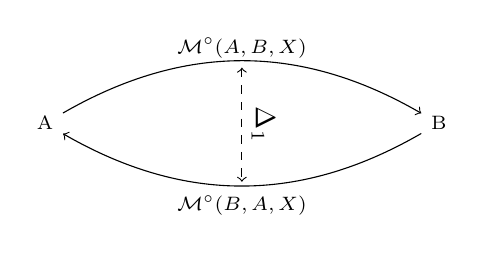
\begin{tikzpicture}[scale=0.5]

\draw(0,0) node[anchor=north] (A) {\scriptsize A};
\draw(10,0) node[anchor=north] (B) {\scriptsize B};
\draw(5,2) node[anchor=north] {\scriptsize \Model{A}{ B}{ X}};
\draw(5,-2) node[anchor=north] {\scriptsize \Model{B}{ A}{ X}};
\draw[dashed, <->] (5,1) -- (5,-1.9) node[midway, sloped, above] {$\Delta_1$};
\draw[->] (A) to[bend left] (B);
\draw[->] (B) to[bend left] (A);

\end{tikzpicture}

\caption{The mutual modelling symmetry question $\Delta_1 =  \Delta(\mathcal{M}^{\circ} (A,B,X),
\mathcal{M}^{\circ} (B,A,X))$}

\label{mm_symmetry}
\end{figure}


With triads, we may compute the accuracy of 6 models:
\Model{A}{B}{X}, \Model{B}{A}{X}, \Model{A}{C}{X}, \Model{C}{A}{X},
\Model{C}{B}{X} and \Model{B}{C}{X}. This enables two
triangle questions (see Fig.~\ref{mm_triangles}):

Do A and B have the same accuracy when modeling C? $\Delta_2 =
\Delta(\M{A}{C}{X}, \M{B}{C}{X})$ If it is the same,
$\mathcal{H}_{2}$ and $\mathcal{H}_{3}$ gain over $\mathcal{H}_{1}$

Does C model more accurately A than B? $\Delta_3= \Delta(\M{C}{A}{X},
\M{C}{B}{X})$ A positive answer would support $\mathcal{H}_{3}$.

\begin{figure}[htb]
\centering
\subcaptionbox{}{ 
    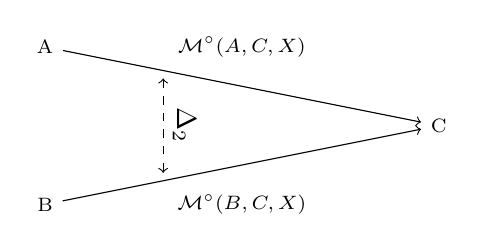
\begin{tikzpicture}[scale=0.5]

    \draw(0,2) node (A) {\scriptsize A};
    \draw(0,-2) node (B) {\scriptsize B};
    \draw(10,0) node (C) {\scriptsize C};

    \draw(5,2) node {\scriptsize \Model{A}{ C}{ X}};
    \draw(5,-2) node {\scriptsize \Model{B}{ C}{ X}};
    \draw[dashed, <->] (3,1.2) -- (3,-1.2) node[midway, sloped, above] {$\Delta_2$};
    \draw[->] (A) to (C);
    \draw[->] (B) to (C);

    \end{tikzpicture}
}
\subcaptionbox{}{ 
    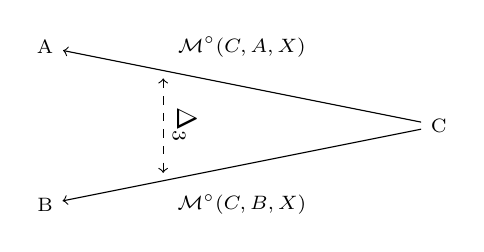
\begin{tikzpicture}[scale=0.5]

    \draw(0,2) node (A) {\scriptsize A};
    \draw(0,-2) node (B) {\scriptsize B};
    \draw(10,0) node (C) {\scriptsize C};

    \draw(5,2) node {\scriptsize \Model{C}{ A}{ X}};
    \draw(5,-2) node {\scriptsize \Model{C}{ B}{ X}};
    \draw[dashed, <->] (3,1.2) -- (3,-1.2) node[midway, sloped, above]
    {$\Delta_3$};
    \draw[<-] (A) to (C);
    \draw[<-] (B) to (C);

    \end{tikzpicture}
}
\caption{The mutual modelling triangle questions}

\label{mm_triangles}
\end{figure}



In addition, the comparison between $\Delta_2$ and $\Delta_3$ could tell us
whether the accuracy of mutual modelling depends more upon the modeller's effort
or the modellee's behaviour.

\paragraph{The rectangle questions}

We could go further by comparing self- versus other modeling $\Delta_4$ in
Fig.~\ref{mm_rectangle}) as an indication of metacognitive skills. We could also
see if modeling skills depend upon what aspects are being modeled (X or Y),
which would explain vertical differences ($\Delta_5$ in
Fig.~\ref{mm_rectangle}). We do not further develop these questions because we
don't have the necessary data in our studies.

\begin{figure}[htb]
\centering

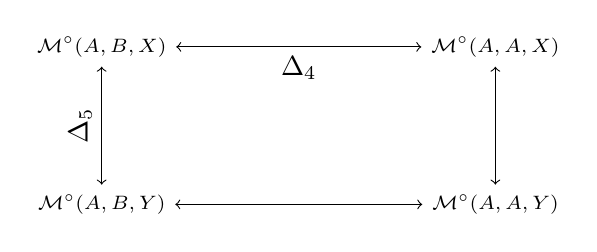
\begin{tikzpicture}[scale=0.5]

    \draw(0,0) node (a) {\scriptsize \Model{A}{ B}{ X}};
    \draw(10,0) node (b) {\scriptsize \Model{A}{ A}{ X}};
    \draw(10,-4) node (c) {\scriptsize \Model{A}{ A}{ Y}};
    \draw(0,-4) node (d) {\scriptsize \Model{A}{ B}{ Y}};
    \draw[<->] (a) -- (b) node[midway, below] {$\Delta_4$};
    \draw[<->] (b) -- (c);
    \draw[<->] (c) -- (d);
    \draw[<->] (d) -- (a) node[midway, sloped, above] {$\Delta_5$};

\end{tikzpicture}

\caption{The rectangle questions}

\label{mm_rectangle}
\end{figure}


This simple notation does not pretend to provide a mathematical account of
mutual modeling but to be more systematic in describing the following
experiments. 




%%%%%%%%%%%%%%%%%%%%%%%%%%%%%%%%%%%%%%%%%%%%%%%%%%%%%%%%%%%%%%%%%%%%%%%%%%%%%%%%%%
%%%%%%%%%%%%%%%%%%%%%%%%%%%%%%%%%%%%%%%%%%%%%%%%%%%%%%%%%%%%%%%%%%%%%%%%%%%%%%%%%%

\section{Studies}



%%%%%%%%%%%%%%%%%%%%%%%%%%%%%%%%%%%%%%%%%%%%%%%%%%%%%%%%%%%%%%%%%%%%%%%%%%%%%%%%%%
\subsection{Study 1: Effect of an awareness tool on \gModel{A}{B} in a virtual
game}

\subsubsection*{Questions}

We studied the impact of an awareness tool on group performance and mutual
modeling~\cite{nova2007collaboration}. The availability
of an awareness tool was our independent variable. In previous studies, we
replayed a video of the game to subjects who surprised us by their ability to
remember former states of their mutual model: ``I did that because I thought that
you would do that''. Hence, this experiment focused the representation of each
other's action plans. During the game, we asked them to anticipate the next
action of their partner as well as to announce their own action. It is clear
asking them a question about their partner increases their attention for the
rest of the game.

\subsubsection*{Experimental setting}

SpaceMiners is a 3D game that involves two players collecting minerals located
in asteroids (Fig.~\ref{study1:spaceminer}). To do so, they shoot drones through the space after choosing their
initial direction and speed. Once launched, the trajectory of drones is only
influenced by the gravity of planets and by trajectory modification tools.
During the experiment, the teams were confronted with three increasingly complex
situations. The experiment was 2 hours long: a 30 minutes tutorial and 3 levels
of 30 minutes. Players uses using a regular joystick and communicated with each
other through an audio channel.

The independent variable was the availability of an awareness tool that shows to
player A  the location and gaze direction of player B. In the awareness
condition, players could switch to the \emph{scout mode} where they could view what
their partner was looking at. We hypothesize that this would enable subjects to
more accurately infer their teammate's intentions. Each player sat in front of a
distinct computer located in different rooms. 

\subsubsection*{Subjects}

Thirty-six persons participated in this study, all native French speakers. We
constituted 18 pairs of participants (N = 18) who were not familiar with each
other. The pairs were assigned randomly to either the control condition (without
the awareness tool) or the awareness condition (with the awareness tool).

\begin{figure*}
        \centering
        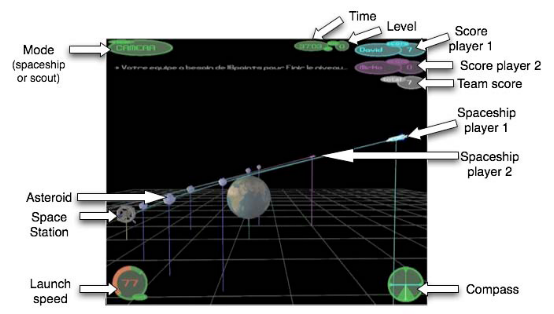
\includegraphics[width=0.9\textwidth]{image4.png}
        \caption{Snapshot of the SpaceMiner Game}
        \label{study1:spaceminer}
\end{figure*}

\subsubsection*{Variables}

Task performance was measured by the score reached by the two subjects after
three situations. The effort of mutual modeling was measured as the ratio of
time that players would spend in the scout mode (divided by total time), which
is the time during which players are not performing their own actions but
monitoring their partner's actions.

In order to evaluate \gModel{A}{B} during the task, we used two questionnaires
(Fig.~\ref{study1:questionnaires}) that were displayed during each of the three
games, as a transparent layer appearing over the game display. The first
questionnaire concerned the player's intended actions. The second questionnaire
asked each player about what he thought her or his partner was intending to do.
Some answers were identical in both questionnaires (like ``adjusting a shot'')
while others were reversed (``to guide my partner'' versus ``to guide me''). We
chose this subjective measure of accuracy ($\Delta(\M{A}{B}{x}, \M{B}{B}{x})$)
rather than an objective measure (\ie the model \gmodel{A}{B} is compared to B's
next action) because some the activities proposed by the questionnaire were not
observable by the environment (\eg establishing a strategy). We counted
\Model{A}{B}{activity_{game_{i}}}) as the number of common answers between
questionnaires \gmodel{A}{B} and \gmodel{B}{B} in each game and computed the
average value a across the 3 games.

\begin{figure}[ht!]
        \centering
        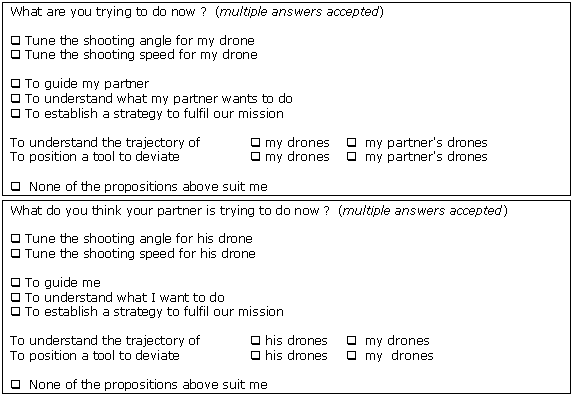
\includegraphics[width=\columnwidth]{image5.png}
        \caption{\gmodel{A}{A} and \gmodel{A}{B} questionnaires in SpaceMiners
        (translated from French).}

        \label{study1:questionnaires}
\end{figure}

\subsubsection*{Results}

\paragraph{Grounding criterion} The grounding criterion was high: the
correlation between \gModel{A}{B} and task performance was 0.42, $p = 0.05$.
Pairs with an accurate mutual model reached higher scores. A regression analysis
confirmed the positive and significant relation between group performance and
mutual modelling accuracy ($\beta=54, p = .02$).

\paragraph{Study-specific questions} The awareness tool permitted higher group
performance, but it did not improve the accuracy of the mutual model. Since
teams were free to use the awareness tool or not (the \emph{scout} mode), we
performed a post-hoc split of players depending on how much time they used it.
The split point was the mean of time spent in the scout mode and it led to the
constitution of two groups made up of 12 individuals ``short time in scout
mode'' and 24 individuals ``long time in scout mode''. A two-way analysis of
variance conducted on these contrasted groups revealed that pairs in the
awareness condition who spent more time in the scout mode reached higher levels
of \gModel{A}{B}($F = 8.02, p = 0.015$). Of course, a \textit{post-hoc} split
does not support a causal direction. An alternative explanation could be that
good modellers are more social and hence appreciate the awareness tool.

\paragraph{Symmetry question} We computed intra-class correlation as described
by~\cite{kenny1998data} from the answers to the cross-questionnaires.
Considering all pairs in both conditions, we found a positive and significant
correlation ($r = .38, p < .05$) between \gModel{A}{B} and \gModel{B}{A}.
Interestingly, this was higher in the control group ($r = 0.44$) than in the
experimental group ($r = 0.24$). Actually, $\Delta(\gMdeg{A}{B},\gMdeg{B}{A})$,
\ie the absolute differences between the models accuracy, was not significantly
different with or without the awareness tool ($F [1,13]= 0.144, p > 0.5$). This
result could be explained by the fact that the players without awareness tools
communicated more.

\paragraph{Triangle questions} We cannot answer the triangle questions since
this study was conducted with dyads.

\subsubsection*{Discussion}

How to interpret a correlation of 0.38 between \gModel{A}{B} and \gModel{B}{A}?
If it was null, modelling would be interpreted as an individual process that
varies according to personality traits or cognitive skills: some persons tend to
model more accurately their peer while others don't care or can simply not. If
the correlation was close to 1, we could conclude that the modelling accuracy is
an emergent property of teams since there would be low probability that, by
chance, low accurate modellers are paired with accurate modellers and
conversely. Our correlation is between these two extremes but the very notion of
significant intra-class correlation tend to indicate that one may not consider
peers as independent subjects, which is an argument for the \emph{interaction}
hypothesis $\mathcal{H}_{3}$. 





%%%%%%%%%%%%%%%%%%%%%%%%%%%%%%%%%%%%%%%%%%%%%%%%%%%%%%%%%%%%%%%%%%%%%%%%%%%%%%%%%%
\subsection{Study 2: Effect of an awareness tool on \gModel{A}{B}  in a pervasive
game}

\subsubsection*{Questions}

This study concerns a collaborative game that occurred in the physical
space~\cite{nova2006underwhelming}. We studied whether players build an accurate
model of the path followed by their partners because this path reflected their
problem solving strategy. We used an objective measure of \gModel{A}{B}: the
distance between where A believes B has been walking and where B actually went.
The main hypothesis concerned the effect of awareness tools on group performance
and on \gModel{A}{B}. 

\subsubsection*{Experimental setting}

{\sc CatchBob} is a mobile game in which groups of 3 players have to solve a
joint task. The game was played on EPFL campus. Participants had to find a
virtual object (\emph{Bob}) and ``to catch it'' by forming a triangle around it.
Players used a Tablet PC that displayed a map of the campus and an indication of
their personal distance to Bob. Their annotations on the map were shared with
the two other players (A could see what B and C wrote). These annotations faded
out after a few minutes to avoid covering the full display. The awareness tool
displayed as well the location of the two other players on the map. The
availability of location awareness tool constituted our independent variable.

\begin{figure*}[h!t]
        \centering
        \begin{subfigure}{.3\textwidth}
            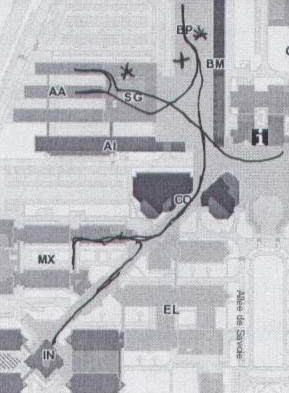
\includegraphics[width=\linewidth]{image6.png}
            \caption{A's drawing of B's path.}
        \end{subfigure}
        \begin{subfigure}{.3\textwidth}
            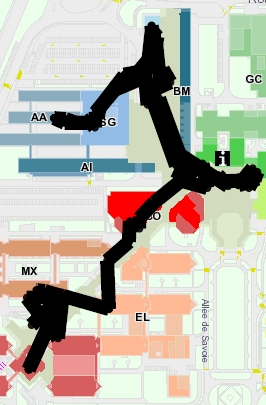
\includegraphics[width=\linewidth]{image7.png}
            \caption{Actual path followed by B.}
        \end{subfigure}
        \caption{Reported and actual path of one of the player, during the {\sc
        CatchBob} game.}
        \label{study2:paths}
\end{figure*}

\subsubsection*{Subjects}

Ninety students participated in this experiment. We chosen only students from
our university because knowing the campus geography had an impact both on group
performance but also on mutual modeling: it is hard to represent the path of
someone across some space without having a mental map of this space. We selected
groups of students who knew each other. We assigned 10 triads to each of our
three experimental conditions. Each condition was made up of approximately 25\%
of women, but we did not control gender repartition within each triad.

\subsubsection*{Variables}

The independent variable was the awareness tool: the control condition (without
tool) and two experimental conditions: synchronous awareness (display current
position of each player) and asynchronous awareness (display current position of
each player and their recent spatial trace).  As a dependent variable, we had
the task performance which was the distance covered by the team to catch Bob and
\gModel{A}{B}. To estimate \gModel{A}{B}, we asked players to draw on paper
their own path and the path of each of their partners after the game. This
enabled us to calculate the number of errors players made while drawing the path
of their partners. We compared the path that player A attributed to B with B's
real path recorded by the system and the same for A \& C and B \& C as depicted
on Fig.~\ref{study2:paths}. 

\gModel{A}{B} is the sum of errors made by A about B's paths. An error was
either drawing a place where the partner had not been or not drawing a place
where he/she had gone. One could argue that \gModel{A}{B} is biased by the
subjects' ability to translate their trajectories souvenir into a map drawing.
However, 85\% of subjects made no mistake at all when drawing their own path. We
therefore consider mistakes in their partners' path as being due to a lack of
mutual modeling accuracy instead of being due to spatial reasoning skills.

\subsubsection*{Results}

\paragraph{Grounding criterion} The correlation between \gModel{A}{B} and the
task performance (path lengths) was low: 0.15. Using a \emph{post-hoc} split on
\gModel{A}{B}, there is no significant difference between the performance of the
groups with high and low \gModel{A}{B}  ($F = 1.45, p = 0.24$). Conversely, a
\emph{post-hoc} split of the groups according to their performance did not show
any significant differences on \gModel{A}{B} ($F = 1.16, p = 0.29$).

\paragraph{Study-specific questions} There was no significant difference
regarding the task performance. However, our surprise was that the absence of
the awareness tool was related to a higher \gModel{A}{B}: players better
remembered their partners' path if they did not see their position permanently!
We will not enter into the details of these results but, to be short, teams
without awareness tool made more annotations on the map while permanent MLA has
an underwhelming effect~\cite{nova2005location}.

\paragraph{Symmetry question} The correlation between \gModel{A}{B}  and
\gModel{B}{A}  is positive ($r = .41$) and significant ($p < .01$);  the more A
makes errors about B, the more B does the same.

\paragraph{Triangle questions} Regarding $\Delta_2$, the correlation between
\gModel{A}{B} and \gModel{A}{C} is significant: $r=0.30, p <.01$. Concerning
$\Delta_3$, the correlation between \gModel{A}{C} and \gModel{B}{C} is
significant as well: $r=0.43, p <.001$.

\subsubsection*{Discussion}

This positive result regarding to the symmetry question is even more surprising
than the previous one: despite the high heterogeneity of spatial skills among
adults~\cite{liben1981spatial}, a significant correlation could indicate that
mutual modeling relies more on group processes than on individual processes. The
significant results on the triangle questions probably go in the same direction:
either the modeler or the modeled both contribute to accurate modeling, or that
the quality of teamwork has a global effect. In this experiment, since team
members did not interact intensively during the task, the factor that
facilitates accurate mutual modeling is probably less the quality of verbal
interactions that the group strategy: a clear strategy facilitates memorizing
one's partner path. 




%%%%%%%%%%%%%%%%%%%%%%%%%%%%%%%%%%%%%%%%%%%%%%%%%%%%%%%%%%%%%%%%%%%%%%%%%%%%%%%%%%
\subsection{Study 3:  Effect of media richness on \gModel{A}{B} in argumentation}

\subsubsection*{Questions}

The aim of this unpublished study was to evaluate the effect of media richness
on \Model{A}{B}{emotions}. The hypothesis was that video communication would
lead to a better \gModel{A}{B} than audio only since emotions often impact on
facial expressions.

\begin{figure*}[ht!]
        \centering
        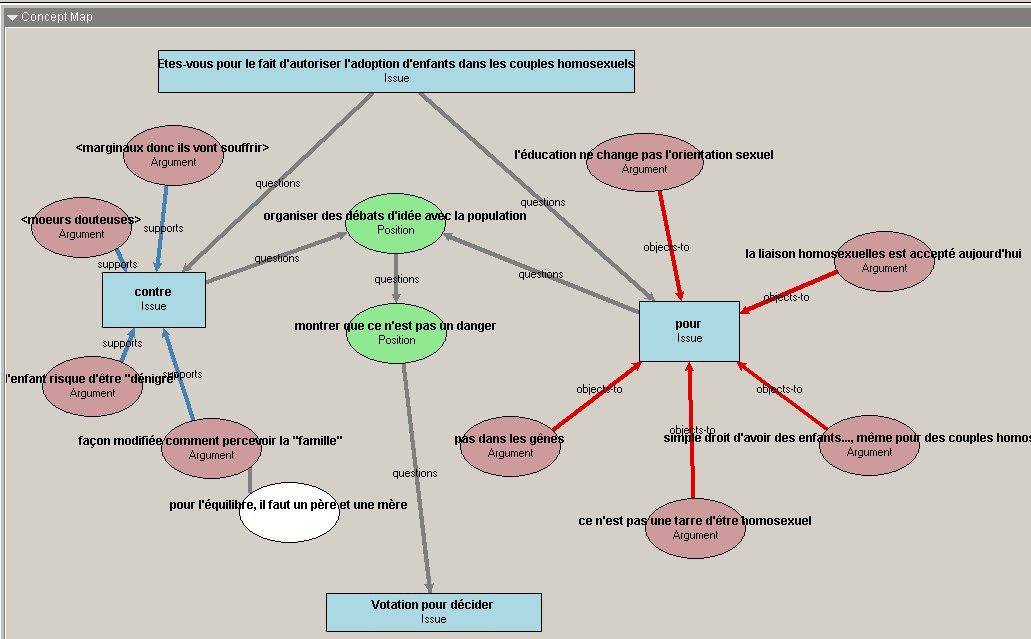
\includegraphics[width=0.9\textwidth]{image8.jpg}
        \caption{Example of argumentation graph}
        \label{study3:argumentation_graph}
\end{figure*}


\subsubsection*{Experimental settings} 

Triads had to address an emotional societal debate: authorizing or not adoption
by homosexual couples. They worked on-line and had to structure their
argumentation with a shared concept map tool {\sc TeamWave} as illustrated in
Fig.~\ref{study3:argumentation_graph}. Ten groups had only an audio connection
while ten groups had audio plus video. The video communication was provided by a
web cam and the software {\sc IVisit}. For the audio link, we used microphones,
headsets and a software called {\sc BattleCom}. In the audio+video condition,
the screen was divided in three sections. The main part was devoted to the
concept map window (24x24cm). In the remaining part appeared the image of the
two peers (8.5x8.5cm each). In the audio condition, this video zone was left
empty so that the size of the concept map was equal in each condition. The
subjects were located in the same room, separated by mobile walls. Despite their
headsets, it is not impossible that they could hear non-verbal audio cues (\eg
tapping the sole with feet).  The task last in average 61 minutes.

\subsubsection*{Subjects}

Twenty triads from the University of Geneva participated to this experiment. We
formed groups of subjects who knew each other, \ie they had \emph{ab initio}
mutual models: the task required the discussion of sensitive issues which
required to feel quite comfortable with peers. There were 36 women and 24 men,
but, since groups were formed a priori, we could not control the balance of men
and women in each condition.

\subsubsection*{Variables}

The independent variable was the presence of not of video link. The dependent
variable \gModel{A}{B} was subjectively by using 3 questionnaires: in the first
one, A described his or her own emotions \gmodel{A}{A} , while in the two other
questionnaire, A describes B's and C's emotions. The questionnaire included 18
items (7-point Likert Scale) describing emotions labeled as adjectives:
\emph{anxious}, \emph{enthusiastic}, \emph{agitated}, \emph{proud},
\emph{excited}, \emph{quiet}, \emph{calm}, \emph{stressed}, \emph{bored},
\emph{upset}, \emph{relaxed}, \emph{irritated}, \emph{determined},
\emph{hostile}, \emph{active}, etc. This list of emotions was
elaborated from \fixme{REF?}. The proposed emotions were \fixme{?}. \gmodel{A}{B} is a vector
of 18 numerical values ${x_1 \dots x_i}$ corresponding to their answers on each
questionnaire. \gModel{A}{B} has been computed as the correlation between the
two vectors (Eq.~\ref{eq:study3}).

\begin{multline} \label{eq:study3}
    \Mdeg{A}{B}{emotions}\\
    = \Delta(\M{A}{B}{\{x_1 \dots x_i\}}, \M{B}{B}{\{y_1 \dots y_i\}}) \\ 
    = r(\{x_1 \dots x_i\}, \{y_1 \dots y_i\})
\end{multline}

\subsubsection*{Results}

\begin{figure*}[ht!]
        \centering
        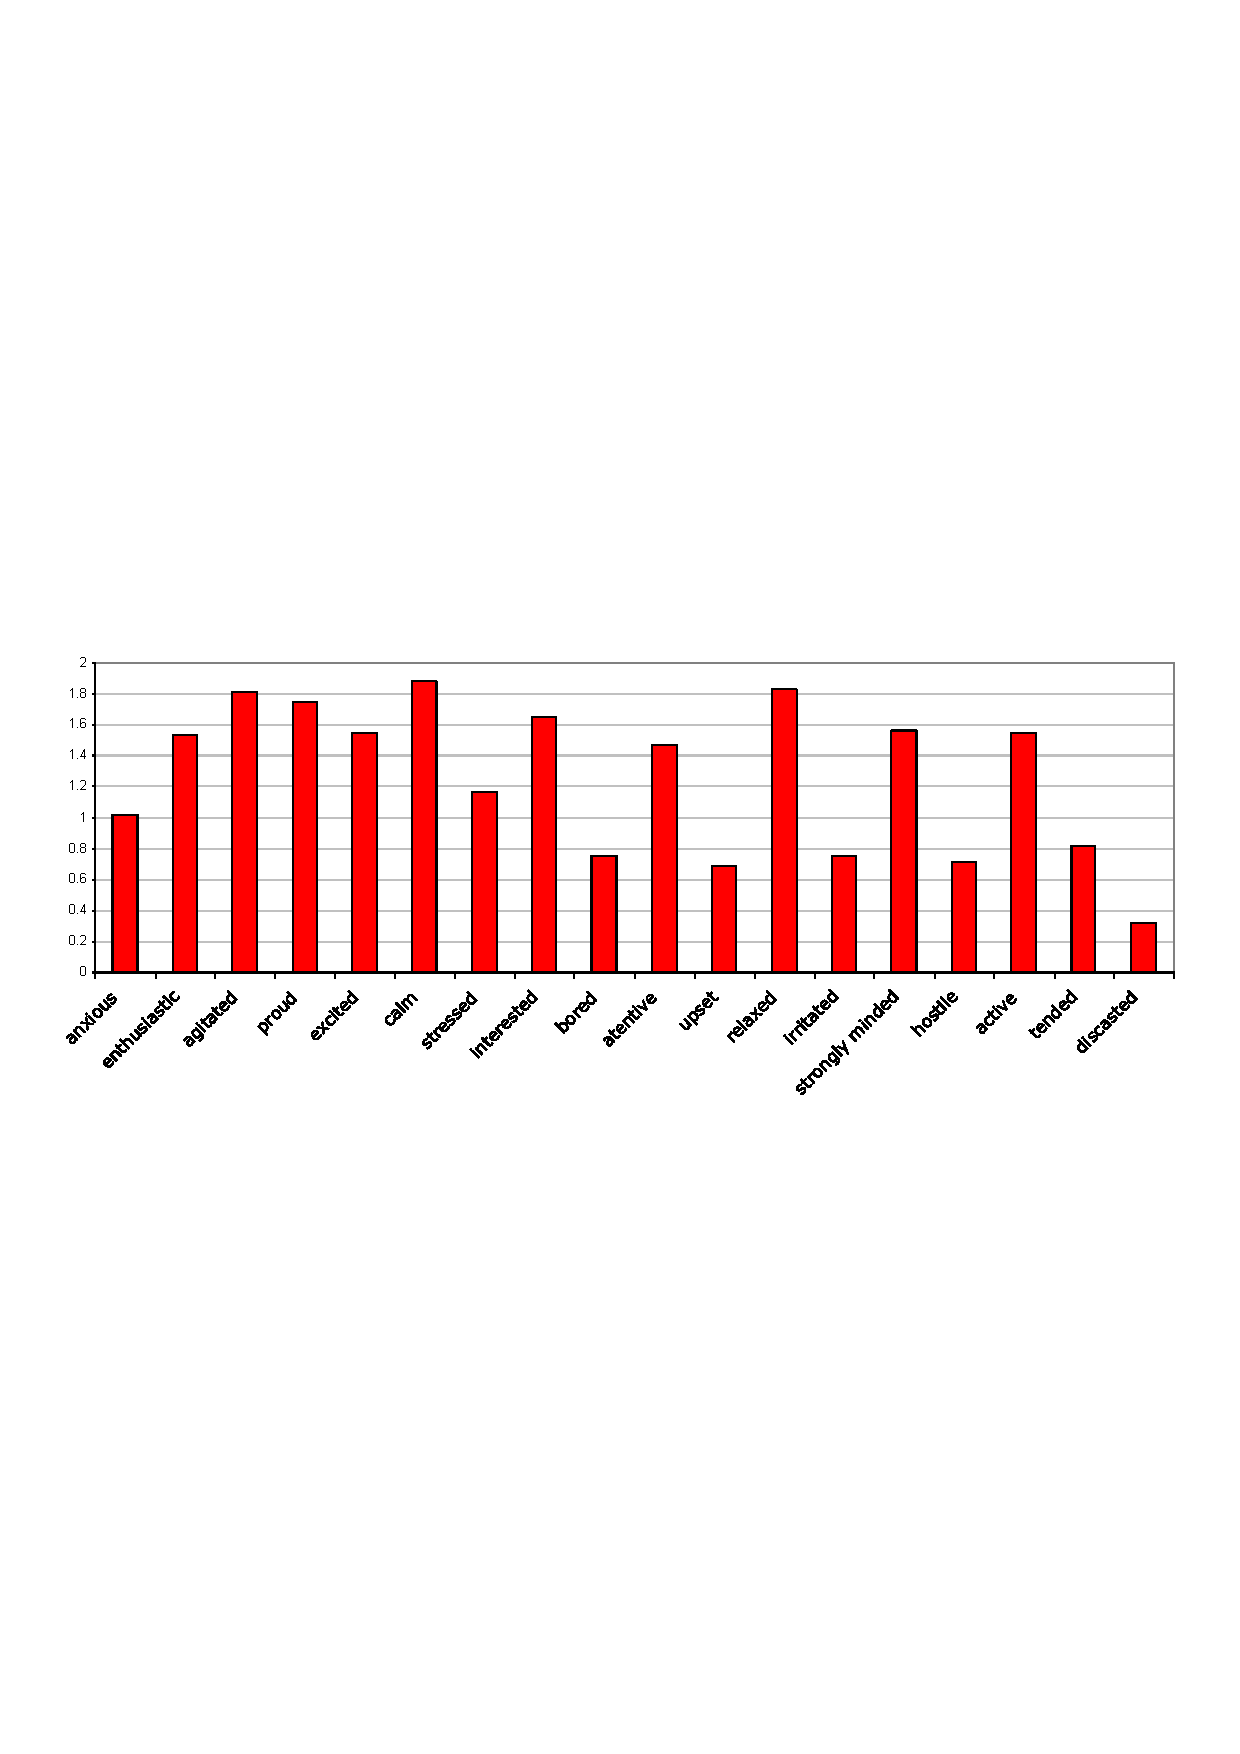
\includegraphics[width=0.9\textwidth]{image9.pdf}
        \caption{Average values of \Model{A}{B}{X} where X is one of the proposed
        emotions (max = 7).}
        \label{study3:deg_m_values}
\end{figure*}

\paragraph{Grounding criterion} The maps produced by teams were ranked. We use
the average rank as a estimation of the team performance and correlated with the
average of the 6 values of \gModel{A}{B} per team (\gModel{A}{B}, \gModel{A}{C},
\gModel{B}{A},...): The correlation is -0.22: teams with a good \gModel{A}{B}
team to be better ranked. 

\paragraph{Study-specific questions} Our hypothesis about media richness is
rejected: the average \Model{A}{B}{emotions} was .62 ($SD = .28$) with the
audio+video condition and .71 ($SD = .19$) in the audio condition ($F=3.4, p:
0.065$). Our interpretation is that viewing what one's partner sees (shared
graphical editor) was, in this task, more important than seeing each
other~\cite{gaver1993one}\fixme{check ref with Pierre}\fixme{other cite:
Anderson et al., 2000}.

\paragraph{Symmetry question} Regarding the main items, the mutual modeling of
emotions, the correlation is .25 or .36  \fixme{a reprendre avec - Patrick}

\paragraph{Triangle questions} \fixme{Check ($\Delta_2$)} For $\Delta_3$, if we
compute for each subject A, the correlation between the vectors of emotions in
\gmodel{B}{A} and the vector in \gmodel{C}{A}, and take the average across all
60 subjects, we obtain a very impressive correlation of .66. This average is
about the same in each condition.

\paragraph{Rectangle question} We cannot address the relationship ($\Delta_4$)
between self-and social accuracy here because we don't have an estimation of
self-accuracy: subjects describe their emotions but we have no way to check if
there are correct. However, by measuring \gModel{A}{B} on  18 emotional labels,
we can however have a glimpse about $\Delta_5$: how \Model{A}{B}{X} varies
according to X.  Fig.~\ref{study3:deg_m_values} shows the range of modelling
errors: the difference between \gmodel{A}{B} and \gmodel{B}{A}, on a scale of 7,
is in average of 0.3 for the emotion \emph{discasted}, and up to 1.9 for the
emotion \emph{calm}. This is probably specific to the variety of scales  ($SD=
0-5$ for \emph{discated} versus $SD=.7$ for \emph{calm}), our point is not to
interpret this too far, but to show that there are large varations even with one
area  (perceiving emotions). 

\subsubsection*{Discussion}

\fixme{TBD}
\fixme{Chek si il faut modifier les resultats de la symmetries}




%%%%%%%%%%%%%%%%%%%%%%%%%%%%%%%%%%%%%%%%%%%%%%%%%%%%%%%%%%%%%%%%%%%%%%%%%%%%%%%%%%
\subsection{Study 4:  Effects of a script on \gModel{A}{B}  in concept mapping}

\subsubsection*{Questions}

This study investigated the effect of a collaboration script on collaborative
learning~\cite{molinari2008effects}. The script chosen is a JIGSAW: two students
receive different but complementary subsets of the knowledge (texts) which have
to be integrated to build a shared concept map.  This script increases the
cognitive effort to build the map, not only to recon ciliate the viewpoints of
each team members but, before that, to find out what the other knows. 

\subsubsection*{Experimental settings}

The instructional material consisted of an explanatory text about the
neurophysiologic phenomenon of \emph{action potential}. The text was divided
into 3 chapters. The peers were located in two rooms equipped with the same
computer.  The experimental session lasted around 90 minutes and consisted of 6
phases: Participants used two software components, {\sc
CmapTools}\footnote{\url{http://cmap.ihmc.us/}} and {\sc
TeamSpeak}\footnote{\url{http://www.goteamspeak.com/}}.

\begin{enumerate}

    \item As a pre-test, participants were asked to write down all they knew
        about the neuron and its functioning (5 minutes).

    \item Participants were instructed to read a text (12 minutes). 

    \item Participants were asked to build individually a concept map in order to
        graphically represent what they learnt from the text (10 minutes). 

    \item Dyads had to built a concept map during 20 minutes, communicating by
        audio.  The screen layout was structured into three areas (see Figure 8) 

    \item Participants were invited to individually complete a knowledge test
        (15-20 minutes). 

    \item Participants where asked to estimate their own- and their partner's
        final knowledge in a questionnaire. 

\end{enumerate}



\begin{figure*}
    \centering
    \begin{tikzpicture}[scale=0.8]
        \node[anchor=south west,inner sep=0] at (0,0)
            {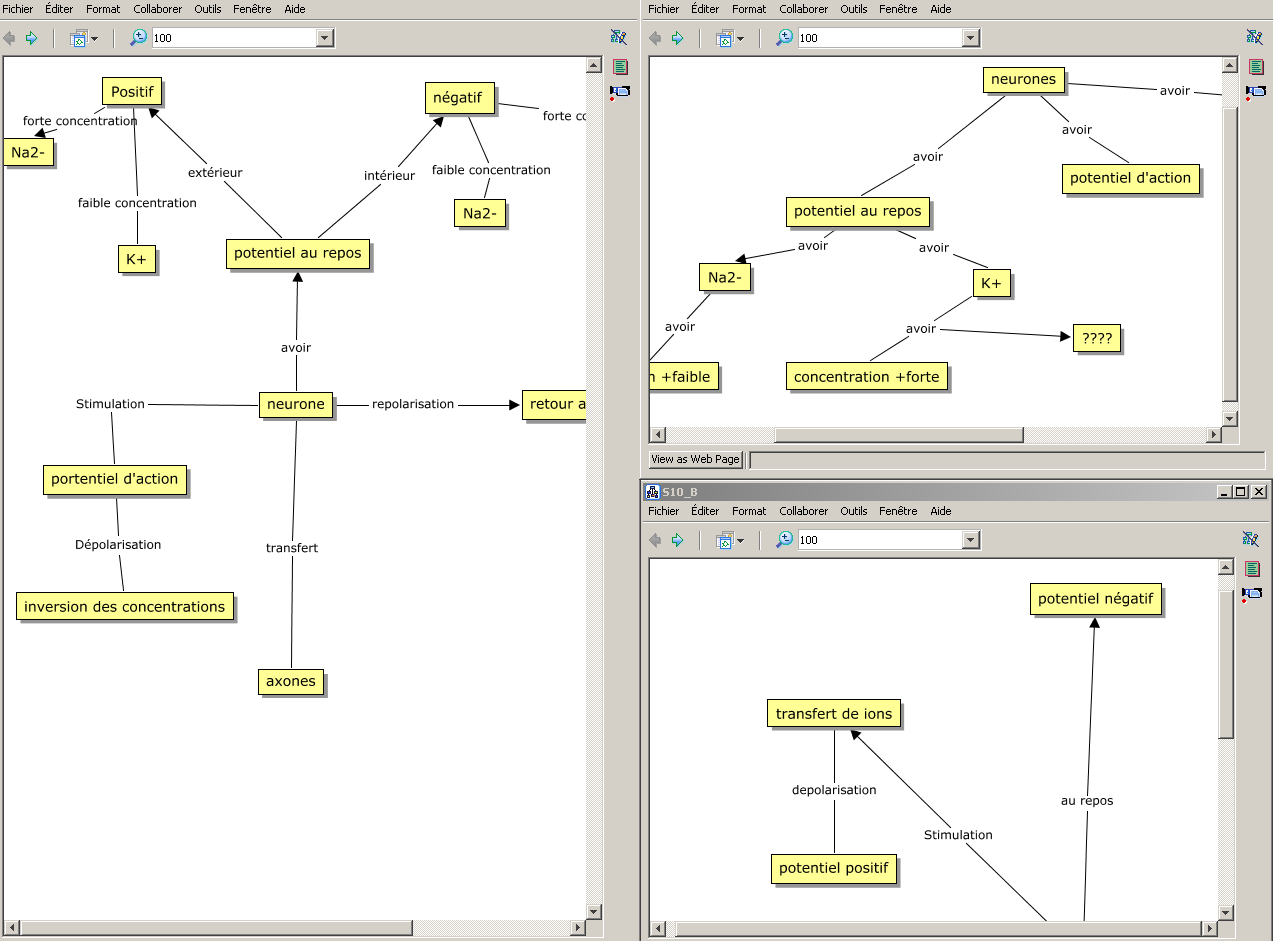
\includegraphics[width=0.65\textwidth]{image10.png}};
        
            \node[rectangle,draw, thick] at (11,6.2) {Self map};
            \node[rectangle,draw, thick] at (11,3) {Partner map};
            \node[rectangle,draw, thick] at (3,2) {Collaborative map};
    \end{tikzpicture}
    \caption{The group concept map and the individual concept maps in study
    4}
    \label{study4:concept_map}
\end{figure*}

\subsubsection*{Subjects}

Fifty-eight first year students from EPFL, 47 men and 11 women, with a mean age
of 20.46 were remunerated for participation. Dyads were randomly assigned to one
of the two experimental conditions. The men/women ratio was equivalent in each
condition. Participants did not know each other before the experiment. Students
from Life Sciences were not recruited since they had too high background
knowledge on the learning domain.

\subsubsection*{Variables}

The independent variable, script versus no-script, was implemented by the
difference of texts that individuals had to read. In the \emph{same information}
(SI) condition, the same text was given to both partners. In the
\emph{complementary information} (CI) condition, it was divided into two
sub-texts, one about the electrical processes of the neuron while the second one
about the chemical processes. These two versions were equivalent in terms of
number of information pieces. 

The dependent variables were the post-test scores, but this paper is mostly
concerned by the \Model{A}{B}{knowledge}. In phase 6, participants were ask to
estimate (7-point Likert scale) their own and their partner's outcome knowledge
with respect to each chapter of the \fixme{zexz}. The order of questions about
oneself and about the other was counterbalanced across participants. We measure
\gModel{A}{B} in an objective (Eq.~\ref{eq:study4.1} and \ref{eq:study4.2}) as
well as in a subjective way (Eq.~\ref{eq:study4.3}).\fixme{check  subjective
assess: 2nd equation?}

\begin{multline} \label{eq:study4.1}
    \Mdeg{A}{B}{knowledge} = \\
        \sum_{i=1}^{3} (\M{A}{B}{chapter_i} - score(B, chapter_i))
\end{multline}

\begin{multline} \label{eq:study4.2}
    \Mdeg{A}{A}{knowledge} = \\
        \sum_{i=1}^{3}  (\M{A}{A}{chapter_i} - score(A, chapter_i))
\end{multline}

\begin{multline} \label{eq:study4.3}
    \Mdeg{A}{B}{knowledge} = \\
        \sum_{i=1}^{3}  (\M{A}{B}{chapter_i} - \M{B}{A}{chapter_i})
\end{multline}

\subsubsection*{Results}

\paragraph{Grounding criterion} In this task, the grounding criterion was low,
but we did not evaluate task performance (\eg the quality of the jointly
produced concept map) but the learning gains. The correlation between
\gModel{A}{B} and A's learning gains is not significant ($\beta =.08, ,NS, N =
60$). It is also not significant within each condition.

\paragraph{Study-specific questions} We performed a non-parametric Mann-Whitney
test on post-test scores for electric questions and a one-way ANOVA on scores
for ionic questions (Levene tests for homogeneity of variances: $p = .02$ and
$ns$, respectively. Results  did not show any significant difference between the
\emph{same information} (SI) condition and the \emph{complementary information}
(CI) condition, neither for electric questions [$U = 388.50, z = -0.88, ns$] nor
for ionic questions [$F(1, 58) = 0.17, ns$].  The effect of scripts on
\gModel{A}{B} was not significant ($F(1, 58) = 0.78, ns$) when considering the
absolute difference between \gModel{A}{B} and B's post-test score. However, A
tended underestimate B's score in the SI condition ($M = -2.06$) and to
overestimate it in the CI condition ($M = 1.21$) ($F(1, 58) = 6.44, p<.01$).
Regarding to \gModel{A}{A}, there was no significant difference between
conditions.

\paragraph{Symmetry question} The interclass correlation between \gModel{A}{B}
and \Model{B}{A} is not significant, but almost ($r=.26, F(1,29)=1.71, p=
0.075$).  Actually, it is significant when students read the same text (SI
condition: $r=0.43, F(1,15)=2.53, p<.05$) but not when they read different texts
($r=.13, F(1,12)=1.3, NS$). 

\paragraph{Triangle questions} Triangle questions do not apply here since we
worked with dyads.

\paragraph{Rectangle question}$\Delta_4$: the correlation between \gmodel{A}{A}
and \gmodel{A}{B} is globally not significant ($r=0.05$) as well as not
significant in each condition: someone good at self-modeling is not necessarily
good at modeling someone else and vice-versa.

\subsubsection*{Discussion}

In this experiment, the symmetry of mutual modelling is only found when subjects
are in conditions of symmetry of information. This consolidates the hypothesis
of \gModel{A}{B} being a property of interactions in context rather than A's
cognitive attitude.



%%%%%%%%%%%%%%%%%%%%%%%%%%%%%%%%%%%%%%%%%%%%%%%%%%%%%%%%%%%%%%%%%%%%%%%%%%%%%%%%%%
\subsection{Study 5: \Model{A}{B}{knowledge} in concept mapping}

\subsubsection*{Questions}

This study investigates if \Model{A}{B}{knowledge} is related to learning
outcomes by comparing teams with or without a knowledge awareness tool (KAT),
\ie a tool that informs A about B's knowledge as measured through a pre-test.

\subsubsection*{Experimental setting}

The peers were located into two different rooms. A complete description of the
study is provided in~\cite{sangin2008learners}. The experiment lasted 90 minutes.

It started with the same two steps as in study 4, followed by:

\begin{enumerate}
    \setcounter{enumi}{2}

    \item Subjects passed a pre-test, with ten questions per chapter. 

    \item Participants had 20 minutes to draw a collaborative concept map
        reporting the content of the texts. They were able to communicate
        orally through headsets.  We used Tobbii eye tracking devices to
        record their gazes.

    \item The post-test included the same items than the pre-test but in a
        different order. 

    \item  Finally, participants were asked to estimate their partner's
        knowledge at the post-test for each of the three chapters on a 7-point
        Likert-like survey. 

\end{enumerate}

\begin{figure*}
        \centering
        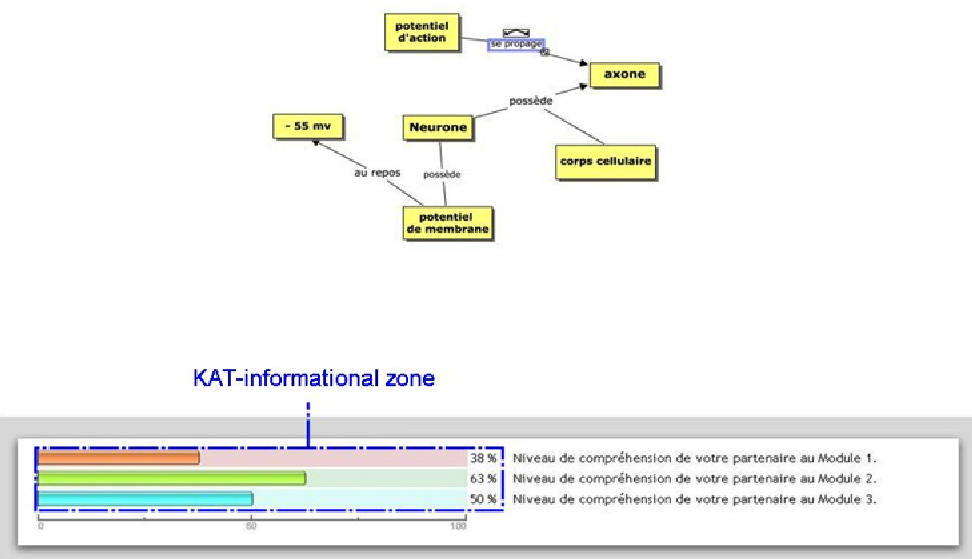
\includegraphics[width=0.9\textwidth]{image11.png}
        \caption{Screenshot of the KAT condition during the concept-map building
        phase.}
        \label{study5:kat}
\end{figure*}

\subsubsection*{Subjects}

Sixty-four first year EPFL students (18 women, mean age = 21.2 years)
participated to the study. They were involved in curricula that do not imply
advanced neurophysiologic notions. They were randomly assigned to conditions and
did not know each other before. 

\subsubsection*{Variables}

The participants of the experimental condition group were provided with the KAT
on the bottom part of the screen (Fig.~\ref{study5:kat}): each line represents
the score obtained by the partner at the pre-test for a chapter. Participants
did not see they own score, but they usually started their discussion by
exchanging this information.

\subsubsection*{Results}

\paragraph{Grounding criterion} A linear regression revealed a positive relation
between \gModel{A}{B} and the collaborative learning gain of the pair $\{A,
B\}$: $\beta= .401, p < .001, r2adj. =.15$, large effect. This relationship was
not significant in the previous experiment which as been conducted with the same
task: using the same task should produce the same grounding criterion. This
probably due to the fact that \gModel{A}{B} was influenced by the KAT.

\paragraph{Study-specific questions} The $t$-test reported a significant
difference between the KAT condition participants ($M = 13.4\%$) and the control
group [$M = 3.6\%, t(1, 60) = 2.73, p < .01$, Cohen's $d = 0.7$, medium to large
effect]. Providing learners with cues about the prior-knowledge of their partner
enhances their collaborative learning. As a treatment check, we found a positive
and significant correlation between the amount of gazes on KAT (using eye
tracking devices) and the learning gains ($r(22) = .54, p = .01$). A detailed
analysis revealed that subjects look at KAT to assess their peer's credibility
when (s)he provided new information. 

The KAT has a significant effect on \gModel{A}{B}: peers more accurately
estimated their partners knowledge ($M = 1.11$) than those in the control
condition [$M = .98, t(1, 60) = 3.19, p < .01$, Cohen's $d = 0.83$, large
effect]. This is a trivial result since the KAT provided them with an initial
\gmodel{A}{B}. However, subjects have to predict the post-test score while the
KAT informed them about the pre-test score. Actually, pairs in the KAT condition
produced significantly more instances of 3 specific categories of interactions:
(1) elaborated utterances with rich contents,  (2) utterances asking about the
other's knowledge such as ``Did you understand how transmission works?'' (3)
utterances describing one's own knowledge (\gmodel{A}{A}) such as ``I don't
remember the Ranvier's thing...''. These 3 categories provide different account
of \gModel{A}{B}: (1) as an effect of the quality of interaction, (2) as an
effect of A's effort to model B or (3) as B's effort to give cues to A about his
own knowledge.

We examined \gModel{A}{B} as potentially mediating the effect of the KAT factor
on the relative learning gain. A linear regression confirmed that \gModel{A}{B}
was significantly related to the KAT-factor ($\beta= .381, p < .01, r2 = .15$).
The KAT-factor was also significantly and positively related to the RLG ($\beta=
.332, p < .01, r2 = .11$). We then tested the relation between the independent
variable (KAT) and the dependent variable (gains) when controlling for the
mediating variable (\gModel{A}{B}). A multiple regression showed that the
KAT-factor was no longer a significant predictor ($\beta= .210; p = ns$) whereas
the \gModel{A}{B} was still a significant predictor ($\beta= .32, p < .01$).
Thus, it can be concluded that \gModel{A}{B} mediated the KAT-factor's effect on
the learners' RLG. The Sobel significance test for indirect effects was
significant [$z = 1.99, p < .05$]. 

\paragraph{Symmetry question} We did not find an intra-pair correlation ($ICC =
0.05, NS$).

\paragraph{Rectangle question} $\Delta_4$: the correlation between \gmodel{A}{A} and \gmodel{A}{B} is
\fixme{???  MIRWEIS A FAIRE}.

\subsubsection*{Discussion}

Despite the fact that the learning task was the same as in study 4, the
conditions of collaboration (viewing multiple maps or not) and the conditions
(scripted or not, awareness tool or not) probably explain differences in terms
of mutual modeling.

\section{Synthesis}

Out of 5 studies, 3 revealed a correlation between the model peers built about
each other: when A builds an accurate model of B, B also tends to build an
accurate model of A.  In one study, this was the case only in one condition.
The conclusion is hence that modeling is mutual but only in certain conditions,
summarized in Table~\ref{synthesis_table}.

\begin{table*}[h!t]
\centering
\resizebox{\textwidth}{!}{%
\begin{tabular}{p{3cm}|p{4cm}|p{4cm}|p{4cm}|p{4cm}|p{4cm}}
\textit{}                     & \textbf{Study 1}                 & \textbf{Study 2}                & \textbf{Study 3}          & \textbf{Study 4}          & \textbf{Study 5}             \\ \hline
\textit{Task}                 & Game in virtual Space            & Game in physical Space          & Building an argument map  & Building a concept map    & Building a concept map       \\
\textit{Interactions}         & Audio                            & Written                         & Audio / Video             & Audio                     & Audio                        \\
\textit{Shared Editor}        & 3D Space                         & 2D Map                          & Concept Map               & Concept Map               & Concept Map                  \\
\textit{Group Size}           & 2                                & 3                               & 3                         & 3                         & 3                            \\
\textit{Duration (mean)}      & 90min                            & 16min                           & 61min                     & 90min                     & 90min                        \\
\textit{Awareness tool}       & Partner's position / orientation & Partner's current/past position & -                         & Partner's concept map     & Partner's scores at pre-test \\
\textit{Dependent variable}   & Team/Ind. performance            & Team/Ind. performance           & Team performance          & Team/Ind. knowledge gains & Team/Ind. knowledge gains    \\
\textit{Independent variable} & Awareness tool vs not.           & Awareness tool vs not.          & Audio only vs Audio+Video & Script vs  not            & Awareness tool vs not.       \\
\textit{MM°-DV correlation}   & +0.42                            & +0.15                           & +0.22                     & +0.08                     & +0.40                        \\
\textit{$\Delta_1$}                   & +0.38 (Sig)                      & +0.41 (Sig)                     & ???                       & +0.26 (near SIG)          & +0.05 (non SIG)              \\
\textit{$\Delta_2$}                   &                                  & +0.30                           & +0.43                     &                           &                              \\
\textit{$\Delta_3$}                   &                                  & ???                             & +0.66                     &                           &                              \\
\textit{$\Delta_4$}                   &                                  &                                 &                           & +0.05                     &                             
\end{tabular}
}
\caption{Comparison of the studies}
\label{synthesis_table}
\end{table*}

Coming back to our initial hypotheses, the $\Delta_2$ results in studies 1, 2
and 3 reinforce both $\mathcal{H}_{2}$ and $\mathcal{H}_{3}$. The
\emph{interaction hypothesis} $\mathcal{H}_{3}$ was that the activity of
modeling one's partner is not simply the result of an individual cognitive
effort but overall the side-effect of the quality of interactions. The
\emph{second-order-modeling hypothesis} $\mathcal{H}_{2}$ stated that, if A is
accurate in modeling B, A should notice when B misunderstands A and should be
able to repair. A good modeler would somehow drive the modeling of his or her
partner.  This \emph{drive} will however occur through verbal cues and repairs
and is hence not easy to differentiate from $\mathcal{H}_{3}$.  The
contradictory $\Delta_1$ results in studies 4 (to some extent) and 5 weaken the
hypothesis. 

The triangular questions lead to similar contradictions. The $\Delta_2$
correlation between the \gmodel{A}{C} and \gmodel{B}{C} (studies 2 and 3?)
support $\mathcal{H}_{2}$ if modeling skills were purely individual, there would
be no reason for modeling skills of A and B to be correlated.  The role of C in
\gmodel{A}{C} and \gmodel{B}{C} probably explains this correlation.  Conversely,
the $\Delta_3$ correlation between the \gmodel{A}{B} and \gmodel{A}{C} (studies
3 and 2?) question $\mathcal{H}_{3}$: if the role of the modellee was so
important, it would lead be surprising to have by chance a correlation between
B's and C' ability to drive A's modeling.

In addition, the lack of correlation between \gmodel{A}{A} and \gmodel{A}{B}
($\Delta_2$ in study 4 and study 5) could also contributes to the idea that A's
modeling skills is not the key factor. However, between modeling someone and
modeling oneself, \ie  metacognition, they are so many differences, that we
would hardly conclude from that,

Among these complex results, it is important to stress that, for $\Delta_2$, the
significant correlations are all below .50, not around .90.  So even if all
$\Delta_2$ correlations were significant in all experiments, we would still not
conclude that modelling purely reflects the quality of social interactions.
There is obviously a large part of individual variance; some of us are much
better in modelling peers. This is not new. The contribution of these studies is
rather to establish the importance of team processes on something that a priori
seemed to be more of a personal cognitive skill.  In other words, we stress that
the bottle is half-full. 

These conclusions must be presented with multiple disclaimers. First, they
heavily rely on correlations; hence we cannot identify causal links. Second, we
faced hard methodological issues. Providing learners with on-task questionnaires
introduce a bias: they will pay more attention to their partners in the
remaining time. Providing them with ``after-task'' questionnaires implies mnemonic
and rationalization biases. The nature of mutual modeling implies methodological
challenges that call for new  measurement methods. We have promising results for
using eye tracking methods to address this challenge.

Finally, let us stress the expressions we used, such as \gmodel{A}{B}, do not
imply we have a mechanical view of modeling. It's just a language for referring
to different components of modeling each other in teams.  This simple notation
emerges from the need to compare five mutual modelling studies; it did not
generate a consistent program of consistent studies.  Our results are not very
robust because they emerge from a \emph{post-hoc} reinterpretation of studies
that addressed different research questions (media richness, awareness tools,
scripts,...). This diversity makes our results difficult to integrate, partly
contradictory. Nonetheless, this diversity gives some generalizability: mutual
modelling has been investigated in different contexts (virtual space versus real
space), with different groups sizes (pairs and triads) and different tasks.
Moreover, these results have been found using different methods for measuring
modeling: on-task in study 1 versus off-task in study 2, subjective validation
in study 1 versus objective validation in study 2 (comparing A's model with B's
behavior).

\section*{Acknowledgments}

The experiments were developed with the help of Patrick Jermann,  Fabien
Girardin, Marc-Antoine Nüssli, Thomas Werhle, Yvan Bourquin and  Jeremy Goslin.
The main funding has been provided from a NSF Grant grant \#102511-106940.

%%%%%%%%%%%%%%%%%%%%%%%%%%%%%%%%%%%%%%%%%%%%%%%%%%%%%%%%%%%%%%%%%%%%%%%%%%%%%%%
\bibliographystyle{abbrv}
\bibliography{biblio}



\end{document}

